% !TeX spellcheck = en_GB
% Methods text

\section{Database: AudioSet}
\label{section:audioset}

\subsection{What is AudioSet} \todo{How cite?}

	Audio Set can be described as a sound large-scale dataset that has the intention of putting the availability of audio and image data on the same level. It is composed by a huge variety of manually-annotated audio events and is organized by following an important ontology formed by 632 different audio classes. The data has been extracted from YouTube videos and the labelling process has been based on diverse factors such as metadata, context and content analysis. It has been developed by Google with the purpose of producing an audio event recognizer that can be applied to plenty of acoustic situations coming from the real world \cite{Gemmeke2017}.
	
\subsection{Ontology}
\label{subsecition:ontology}

	In order to put this dataset together the events have been organized in an abstract hierarchy. This is composed by higher-level classes which  describe a certain type of sound and also acts as parents of other labels that refer to more specific events. With this purpose, the relationship among different classes needed to be non-exclusive, so labelling similar audio events may result into a more general class, the parent, if there existed ambiguity. This is also helpful for labellers due to group the clips in an easier and faster way.
	
	The Audio Set Ontology has been made considering some fundamental guidelines as the ones explained below:
	% List
	% !TeX spellcheck = en_GB
\begin{itemize}
	\item \doubt{A complete collection of all labels must be prepared} so that it can be used to define sound events from real-world aural data.
	\item When labelling an audio event the result must match the criteria of a common listener.
	\item Different categories should be easy to distinguish by an ordinary listener. In the case that two different labels do not satisfy this requirement, these should be merged. With this condition, the spectrum of possible labels remains limited.
	\item The distinction of two different classes must be done by relying just on the audio, it cannot be accompanied by image or visual information.
	\item The hierarchy should not be very deep by keeping the number of children per parent class to no more than 10. This also eases the annotation labour. 
\end{itemize}

	
	It is easy that an ontology of this volume gets leaned or biased in a particular direction due to several factors, such as the subjectiveness of its creators or the selection of the initial set of classes used when starting to work. With the intention of generating a primary list that covers a wide range of audio events in an objective way, the researchers decided to apply an impartial, web-scale text analysis from the very beginning. They agreed on detecting hyponyms of the word "sound" by utilizing a modified version of the famous technique called \textit{Hearst patterns} \cite{Hearst1992}, a method proposed to automatically acquire hyponymy lexical relations from unrestricted text. As a result, an enormous collection of terms came up. This was filtered by considering how well these terms represented audio, i.e. by combining together the global frequency of occurrence and how exclusively these are recognized as hyponyms of "sound" instead of other terms. As an output of the final process, a list of 3000 terms was obtained.
	
	With respect to the hierarchical relation among categories, it was constructed by the authors with the main intention that this satisfied their human comprehension of the sounds. Event though this is a subjective manner, it also makes sense since this is how the hierarchy best performs its labour on helping human labelling.
	After all the organization process, the model is not based on a strict behaviour as a singular node can appear in many different locations, i.e., a single node can be child of different parent nodes. The final result is composed by 632 audio event labels and, in the hierarchy, there is no deeper case than 6 levels. Figure \ref{fig:mesh1} shows the nodes that belong to the two top layers of the ontology.
	
	% Figure of ontology
	\begin{figure}[h]
		\centering
		\captionsetup{justification=centering}
		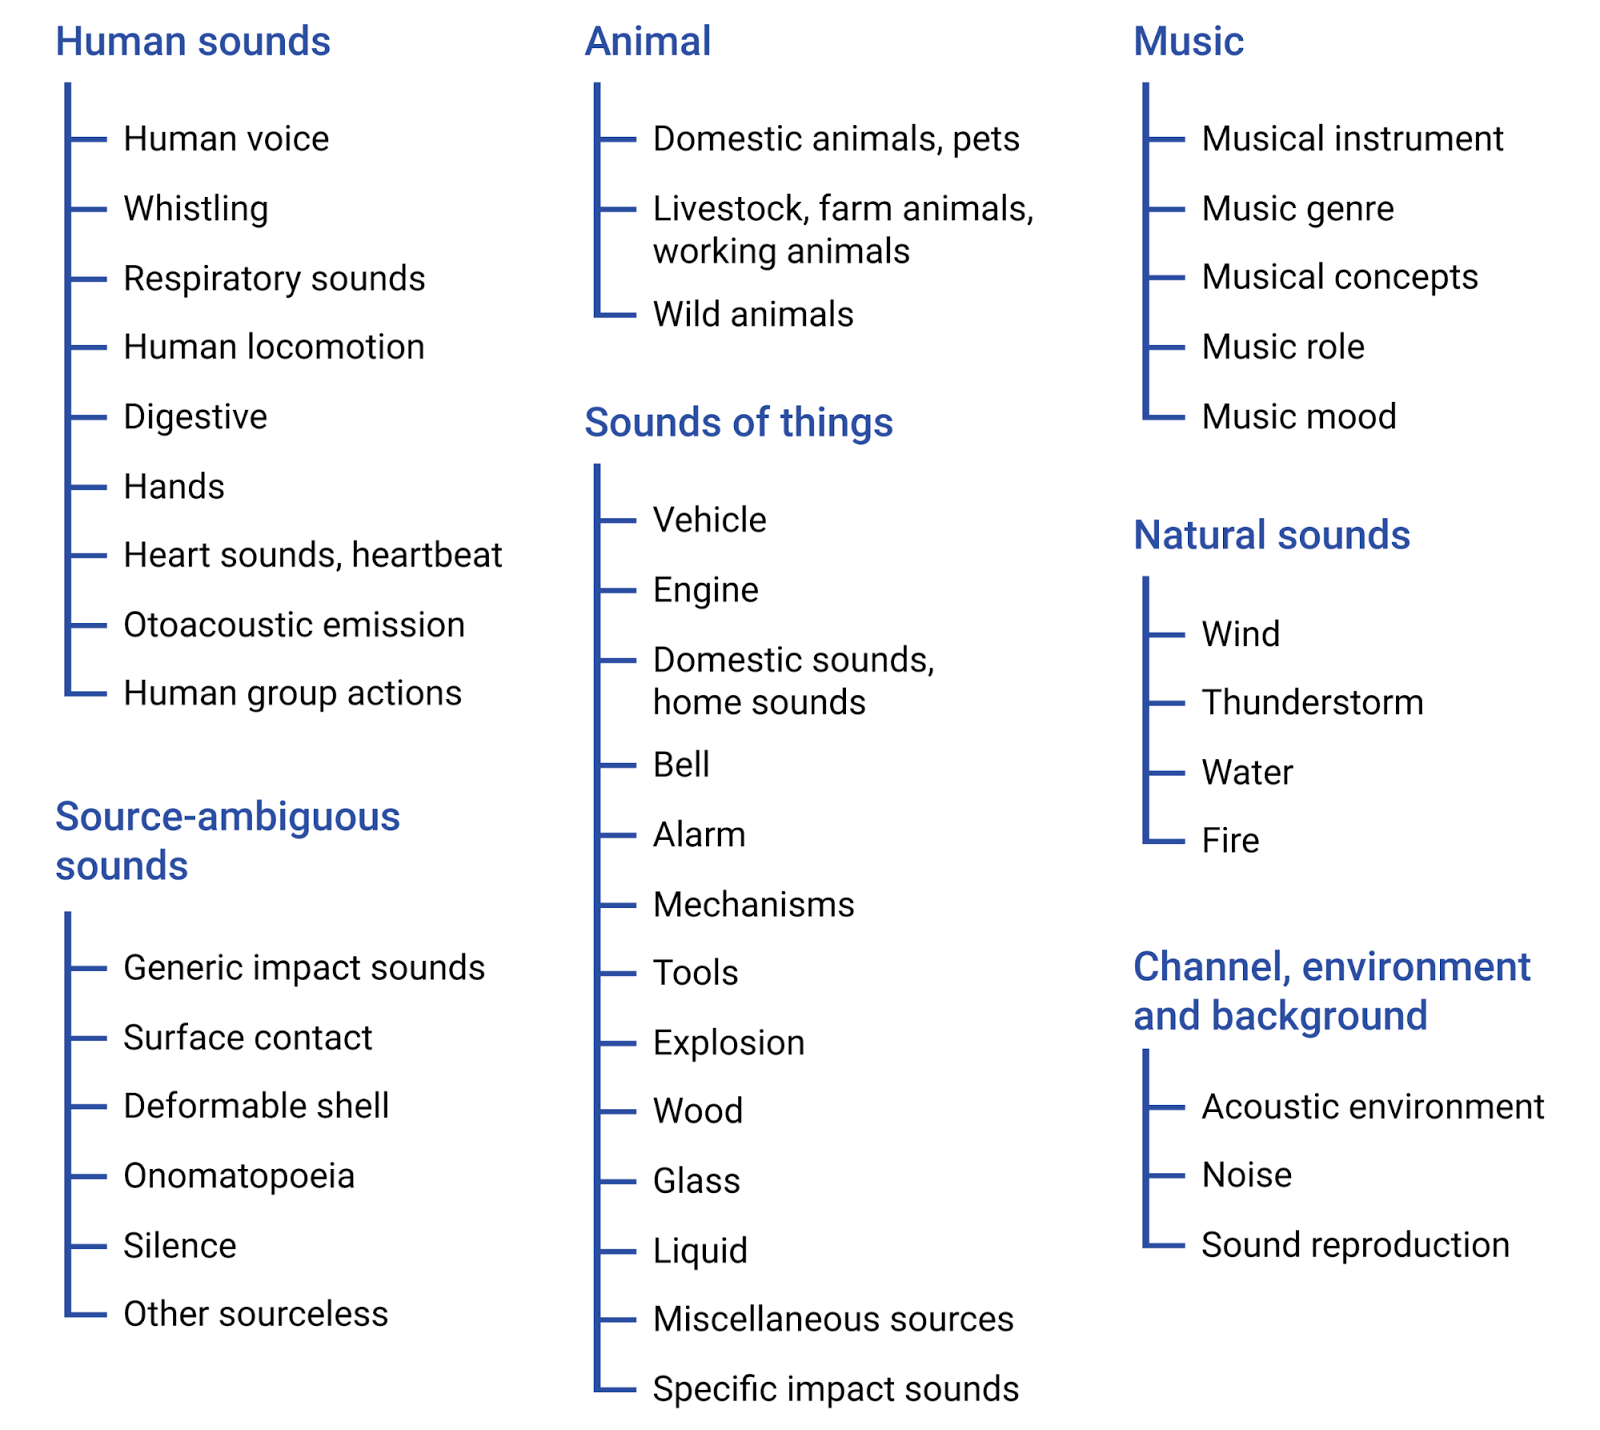
\includegraphics[scale=0.21]{audioset-ontology}
		\caption{First two layers of Audio Set Ontology \cite{Gemmeke2017}}
		\label{fig:mesh1}
	\end{figure}
	
	This whole structure has been given to the user as a file in JSON format. A couple of fields have been included for each label in order to describe its meaning and make clear its position within the hierarchy. A description for all of these can be found in table \ref{table:2}. 
	% !TeX spellcheck = en_GB
% Ontology-fields table

\begin{table}[h!]
\begin{center}
	\begin{tabular}{|| m{7em} | m{22em} ||}
		\hline
		ID & This field includes the Knowledge Graph \acrfull{mid} that best describes the sound or its source. It is used as a primary identifier for the class. \\
		\hline
		Display name & Short name formed by one or two words that identifies the audio class. It sometimes includes a small alternative separated by a comma so it does not feel ambiguous. \\
		\hline
		Description & One or two explaining sentences so the meaning of the category is more defined. These can be extracted from Wikipedia or WordNet. \\
		\hline
		Examples & At least one example of the label is provided as a URL of a YouTube video. \\
		\hline
		Children & An array filled by the \acrfull{mid}s from all immediate children of the class. \\
		\hline
		Restrictions & It specifies if the category in question either has been discarded or there are no audio clips under it. \\
		\hline
	\end{tabular}
\end{center}
\caption{Fields per category in the ontology.}
\label{table:2}
\end{table}
	For the field \textit{ID}, the identifiers are known as \acrfull{mid} and belong to the \textit{Knowledge Graph} designed by Google \cite{Singhal2012}. This is a knowledge base that Google services use to improve the quality of its search results and it is composed with information extracted from a wide variety of sources. The \acrshort{mid}s are the identifiers of the different elements that belong to this huge dictionary. For instance, the \acrshort{mid} of the word "Speech" is "/m/09x0r". Another field that deserves a special explanation is the one corresponding to \textit{Restrictions}. Within all the categories of sound events, there are two flags that indicate an exclusive behaviour that differ from a typical label: "blacklisted" and "abstract". The former refers to a class that has been hidden from labellers due to its confusing meaning. The latter has been used for those classes that are just utilized as intermediate nodes in order to provide a better grouping inside the organization, and are not expected to be used in the implementation tasks. In total, out of the 632 categories, 56 have been categorized as "blacklisted" and 22, as "abstract".
	
\subsection{Data}
\label{subsection:data}

	The different YouTube videos that constitute the dataset are included in a \acrshort{csv} file in which each row is formed by the video identifier, the start and end time of the audio event within the video and the ontology labels that the certain clip belongs to. All the video segments have a longitude of 10 seconds maximum, except from those that the original video is shorter, then the whole thing  will be considered as the an audio event. \todo{Include any explanation about ratings?}
	
	The final release of the dataset is composed by 1,789,621 segments, with a duration of 4,971 hours of video and audio. After executing the selection process in which the different labels were populated with the final corresponding segments, a total of 527 classes were gathered, out of which 485 counted with at least 100 samples.
	
\subsection{Data access}
\label{subsection:data-access}

	The data can be obtained through the website \cite{SoundUnderstandinggroup2017} in two different formats:
	
	\begin{itemize}
		\item Files in \acrshort{csv} format that include for each video segment its YouTube video ID, start time, end time and the one or more labels it belongs to. 
		\item Instead of the audio files themselves, they provide already extracted audio features for each segment in compressed files that can be easily downloaded.
	\end{itemize}

	For our purpose, we worked with the dataset in both different ways. However, we got further with the already extracted features. These are obtained by using a model called \textit{\acrshort{vgg}ish} \cite{Hershey2017} which has been pre trained on a preliminary version of the database YouTube-8M \cite{VideoUnderstandingGroup2017}. The features are available to the user in \acrfull{tf} \cite{GoogleResearch2015} record files and the code for the \acrshort{vgg}ish model is also included in a public repository. \todo{include a type of introduction for vggish?}

\section{Feature extractor}
\label{section:feature-extractor}

	In order to best describe the just mentioned \acrshort{vgg}ish mode, it is necessary to first explain the  original network it was based in. 
	
\subsection{\acrfull{vgg} model}
\label{subsection:vgg}
	
	\acrfull{cnn} are usually able to achieve really good results and even improve human skills on \acrlong{cv} tasks, for example, on recognizing object in an image. With the exponentially growth of the researching works about this field, some challenges have appeared so as to promote the creation of new systems and test their efficiency and results. This is the case of the \acrfull{ilsvrc}, based on the database of the same name, ImageNet. As a solution for the proposed exercise, the investigators from the \acrfull{vgg} in the University of Oxford implemented a new system achieving the first position and winning the challenge in 2014 \cite{ImageNet2014}. The work they proposed consists of a study of the depth in a \acrlong{convnet} architecture and how this can affect to the accuracy on the goal of large-scale image recognition \cite{Simonyan2015}. \todo{Appendix to CNN?} To try this, it was necessary to increase the number of layers in the network, which was viable due to use a small size of convolutional filters in all of them.
	
	For the training step of their system, they used an input image with standard size of $224 \times 224$ in \acrshort{rgb} format. The principles to build the architecture are detailed below:
	
	\begin{itemize}
		\item The input image crosses a bunch of convolutional layers in which the kernel has a size of $3 \times 3$.
		\item The convolutional stride has a value of 1 pixel.
		\item The padding is fixed to 1 pixel, so the dimensions of the input do not change during the convolution.
		\item Max-pooling is also included with a window size of $2 \times 2$ and a stride value of 2 pixels.
		\item Two \acrfull{fc} layers with 4096 channels after all the \acrlong{convnet} layers.
		\item One \acrshort{fc} layer with 1000 channels to perform the \acrshort{ilsvrc} classification.
		\item Soft-max layer for the final layer
		\item All hidden \acrlong{convnet} layers use the non-linear function \acrshort{relu} as \doubt{activation function}.
	\end{itemize}\todo{Normalization?}

	All the designs that the creators came up with are based on these initial guidelines, except from just one case where \acrfull{lrn} is applied.They just differ from each other on the number of layers, starting with 11 the first approach and ending with 19 the last one. The different architectures are specified in the table \ref{table:3} and are ordered from A to E.
	
	% Table configuration of VGG
	\begin{table}[t!]
		\begin{center}
		\captionsetup{justification=centering}
		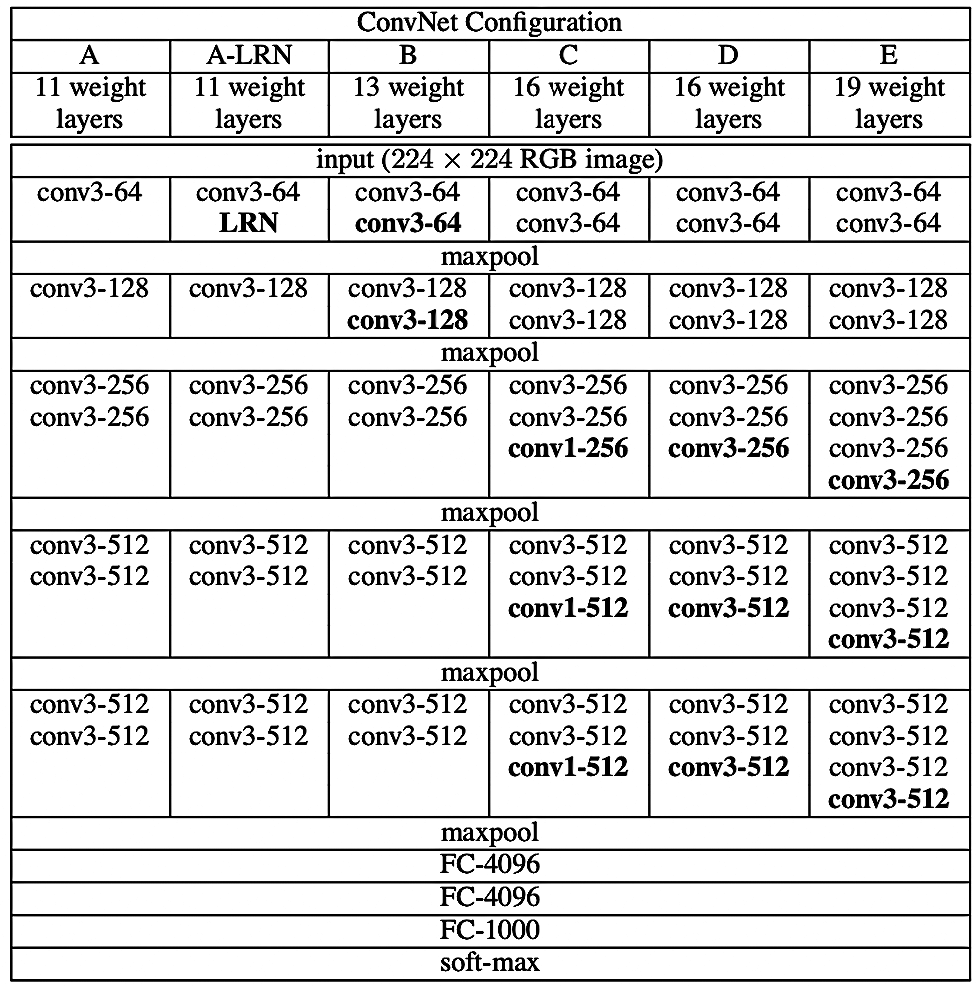
\includegraphics[scale=0.4]{vgg-confs}
		\caption{VGG ConvNet configurations}
		\label{table:3}
		\end{center}
	\end{table}


\subsection{\acrshort{vgg}ish model}
\label{subsection:vggish}
	
	The model we used in our task presents a configuration with principles similar to the ones explained in the previous subsection \ref{subsection:vgg} but with slightly changes that the developers have included in order to adapt it to the audio approach.
	
	The architecture is based in the configuration A from table \ref{table:3} with 11 weights. The differences respect to the original network are listed below: 
	\begin{itemize}
		\item The input size was change from $224 \times 224$ to $96 \times 64$ because of the log-mel spectrogram audio inputs.
		\item They built the implementation with just four groups of convolutional and max-pool layers so the fifth one was dropped.
		\item For the last \acrshort{fc} layer, they decided to build it with just 128 channels since it is the one that compacts the final embedding.
		\item Also the \textit{Softmax} layer is not used.
	\end{itemize}
	In figure \ref{fig:mesh2} is shown how looks the configuration of the final \acrshort{vgg}ish model.
	
	\begin{figure}
		\centering
		\captionsetup{justification=centering}
		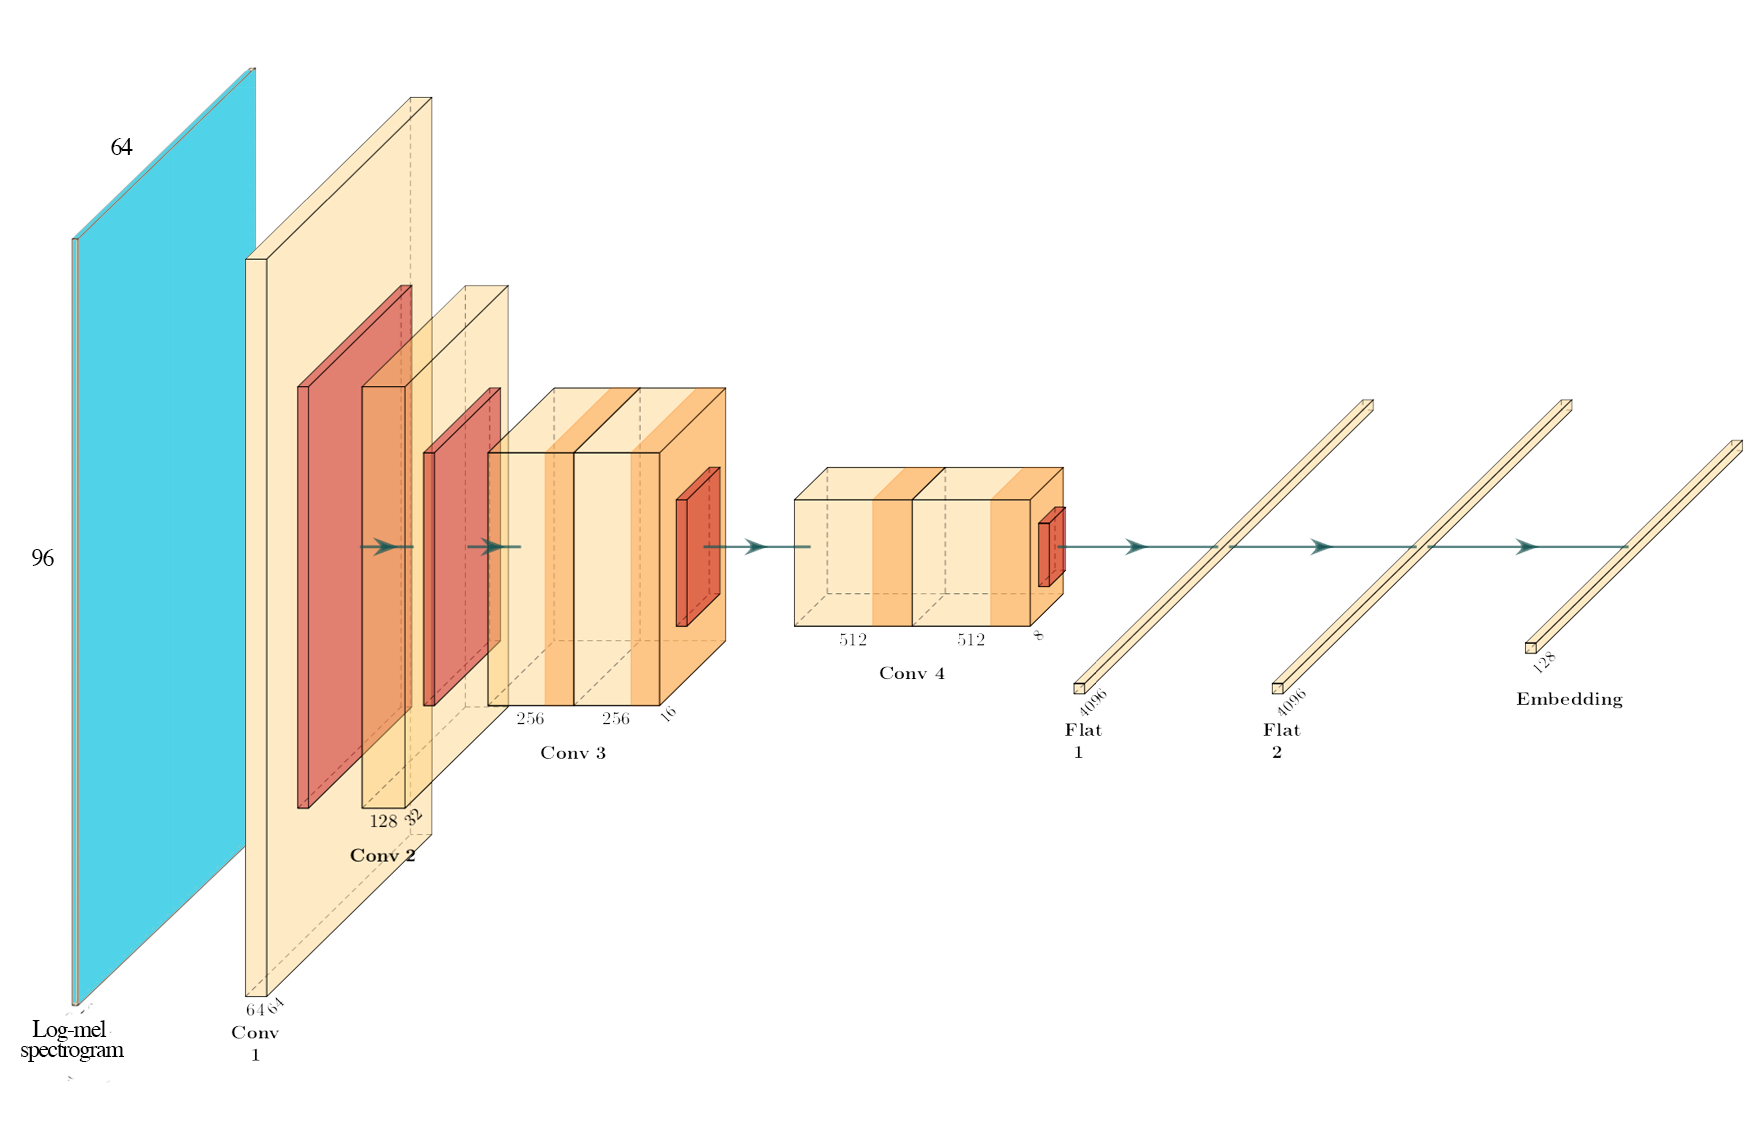
\includegraphics[scale=0.27]{model-vggish}
		\caption{VGGish architecture}
		\label{fig:mesh2}
	\end{figure}

	\subsubsection*{Input stage}
	
	Before passing the data through the whole \acrshort{cnn}, a preprocessing stage have been included by the developers in which the input audio will suffer some transformations. 
	
	\begin{enumerate}
	\item In first place, after loading the input audio, the sample rate and the number of channels are checked to be 16 kHz and monochannel, otherwise the file is transformed to satisfy these conditions.
	\item When the data is ready, the next step is computing the spectrogram. For this, it is necessary to calculate first the \acrfull{stft} of the signal. The operation is performed by using a sliding window of 25 ms of type Hann with a hop size of 10 ms. As a result, just the magnitudes that correspond to the positive frequencies are taken, since the ones corresponding to the negative part of the spectrogram are the conjugate of the others.
	\item  Transforming the spectrogram to Mel scale is what follows. To do so, they compute all mel frequency bins that are going to modify the values of the spectrogram in frequency domain by following a hertz to mel conversion formula \todo{citation?}. The result is a mel spectrogram from 125 Hz to 7,500 Hz divided in 64 bins.
	\item Then, the log-mel spectrogram is calculated by doing the logarithm of the previous result plus a small offset value \doubt{to avoid the logarithm of $0$}.
	\item As a final step, they compute a framing operation over the log-mel spectrogram. The resulting are non-overlapping examples of 0.96 seconds, in which 64 mel bands and 96 frames are contained, each frame with a duration of 10 ms.
	\end{enumerate}

	Therefore, the result obtained is an ensemble of 10 frames, approximately one per second, each of them with size $96 \times 64$, i.e, 96 frames and 64 mel bands.
	
	\subsubsection*{Embedding stage}
	
	Once the initial processing part is done and the log-mel spectrogram matrix is computed and divided into the desired number of frames, it is used as input data for the \acrshort{vgg}ish \acrshort{cnn}. After all the computations inside the network, each example is converted to an embedding of size 128 giving a result of one of this per second of the original audio file. It is good to mention that in this part, a pre trained checkpoint file is loaded.
	
	\subsubsection*{Postprocessing stage}
	
	As final step, they performed some processing of the resulting embeddings. A \acrfull{pca} transformation is done joint with a whitening process. Also, a quantization to 8 bit for each embedding element. All these actions are computed with the purpose of making the final output compatible with the embeddings obtained from the YouTube-8M database.
	
	\todo{Transfer learning and why choosing this type}
	
\subsection{Why \acrshort{vgg}ish}

	For our goal, one of the toughest tasks consisted on the selection of data that properly adapted to our problem and its preparation so as to obtain features that allowed us to characterize every acoustic event from a violent point of view. Since our first efforts of finding an available dataset characterized for being rich in violent scenes were driving us to a dead end, we decided to take advantage of a huge database which let us rethink the standpoint about how we were going to address the problem. As it was mentioned in subsection \ref{subsection:our-point-of-view}, one of the main questions was how to define the term violence for each victim depending on how her certain situation. After finding the Audio Set database, previously explained in section \ref{section:audioset}, with all its variety of samples, we had a wide range of audio data to work with. This is how we came up with the system explained below in \ref{subsection:violent-classes}.
	
	At this point, not only we had an idea but we had already found a data resource to start with. However, the issue was related to what kind of features could be extracted in order to categorize events from different nature with a unique violent label. An acceptable conception of the term violence could be expected to cover all kind of short high gain events such as hits, smashes, gunshots, yells, etc. Also, we would like to introduce sounds that were likely to happen in a domestic environment within a \doubt{tense} atmosphere as children crying, dog barking or glass breaking. However, we also wanted to take into account the possibility of including other cases not usually consider violent a priori. For example, the sound of keys jangling or the noise produces by a shaver machine. These situations may be too particular and just would be present in few uses, but this is how we understand the problem. So, our first intention was to apply some audio processing techniques to extract low-level features, as the ones previously explained in \ref{subsection:features-and-methods}. Even though there are plenty of previous works and a lot of tools to work in this way, it was not sure which path should we had to take in order to decide what features better fitted our task. Apart from this, since the database had such a big volume it would have supposed an enormous cost of time to compute features every time we wanted to try new type of categories. Moving on, by following the advances on finding new level features already mentioned in \ref{subsection:features-and-methods}, we decided to investigate new methods of extraction based on the use of \acrlong{nn} models. Nevertheless, even thought the features obtained in this case had been more appropriated, the time consumption of training a big model was one of the aspects that did not totally convince us.
	
	The previous selection of Audio Set as our dataset allowed us to get to know the \acrshort{vgg}ish model proposed by Google researchers for feature extraction. This system loads the parameters already learned from training with another huge dataset as YouTube-8M. This is possible due to apply transfer learning idea, explained above in subsection \ref{subsection:transfer-learning}, that consists of leveraging features or weights extracted from certain models and use them in simpler ways for different tasks \cite{Sarkar2018}, so all the computational cost and training time is not a problem anymore. Finally, we decided to put in practice this pre trained embedding extractor by loading the given parameters so as to obtain our final input representations.
	
\section{Our approach}
\label{section:our-approach}

	In order to start describing our approach, we will first explain in \ref{subsection:input-data} how we obtained the input data to work with by using the resources previously explained in \ref{section:audioset} and \ref{section:feature-extractor}, and then we will move to the implementation of the whole model in section \ref{}.
	
\subsection{Input data}
\label{subsection:input-data}

	Different phases took place when trying to obtain all the necessary data from the YouTube videos specified in the database. We will explain them from the first step of deciding which classes better fit our problem to the last part in which the desired embeddings are achieved.
	
\subsubsection{Violent classes}
\label{subsection:violent-classes}

	In subsection \ref{subsection:our-point-of-view} it is mentioned our idea about giving the victim the right of defining her own perception of violence, so the final machine can adapt to her situation in a better way. To do so, we have taken advantage of the ontology provided by the Audio Set creators that is properly explained in subsection \ref{subsecition:ontology}. 
	
	Our little system has been implemented based on the idea of using the parent-children relationship among the different nodes. It must go through all the branches so as to offer the victim the possibility of choosing any of the audio event categories. However, instead of consider each label individually, this starts the way from the parent classes down to the children ones.
	
	% Flowchart of user interact system
	\begin{wrapfigure}{R}{0.4\textwidth}
		\centering
		\captionsetup{justification=centering}
		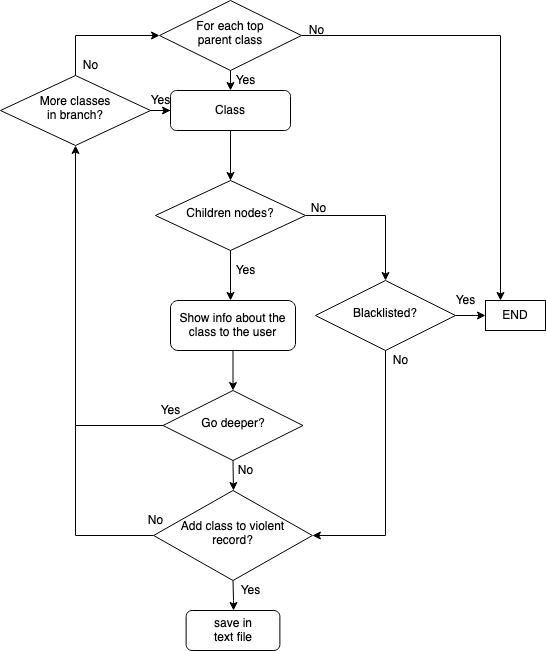
\includegraphics[scale=0.4]{select-vio-cls}
		\caption{Flowchart about selecting violent classes}
		\label{fig:mesh3}
	\end{wrapfigure}
	
	
	Let's say we begin from the class "Human sounds" that is the top level of all sounds emitted by humans contained in the dataset. The system will ask the user if she wants to advance in that direction, i.e., to go across the branches that belong to that part of the \doubt{tree}. If the answer is positive, it would go for the next class, that in this case it would be "Human Speech". It will advance this way until there were no children nodes in the actual class. When this happens, the user will be asked for adding the label to the record of \textit{violent classes}, that will be saved in a text file so they can be read by other parts of the model further on. If the user does not want to go deeper, she will be asked to add the current class to the record. If the answer is "No", then they system will jump to the next sibling category. The corresponding flowchart is shown in figure \ref{fig:mesh3}.
	
	This way of flowing through the different classes allows to skip those parts that does not really relate to our problem. For example, as we can see in figure \ref{fig:mesh1}, one of the top parent labels is "Natural sounds", that relates to sounds from weather phenomena. In most of the cases these classes will not be selected so the whole branch can be skipped. 
	
\subsubsection{Downloading videos}

	The following step consists in achieving audio files that belong to the chosen labels. For this purpose, we have made use of the \acrshort{csv} files that were explained in subsection \ref{subsection:data-access}. For each included video, we took its ID and build the corresponding YouTube \acrshort{url}. Once downloaded, we trimmed the file considering the onset and offset and, finally, converted to audio format (\acrshort{wav}). In our script, we can pass as a parameter the identifier of the desired classes in comma-separated format and either the number of videos per class for a balanced set or a total number of downloads for an unbalanced set. However, there might be some errors when obtaining all the data. The two most common cases are due to lack of enough videos of the desired type in the dataset or because the video is not available anymore on YouTube. When this happens, a message will be shown to the user.
	
	It may also need to be mentioned that throughout the developing of this downloading task, a script has been coded to achieve the whole dataset in both formats, video and audio, for future works. We are not going to specify anything else since it was not finally used.
	
\subsection{Extracting embeddings}
\label{subsection:extracting-embeddings}

	At this point, all the desired data has been already achieved to extract the embedded features that will be used to train the model. For this part, we have used the \acrshort{vgg}ish network explained in subsection \ref{subsection:vggish}. Sine the audio files duration is usually 10 s, and the embedding extractor gives as a result a vector of size $1 \times 128$ for each second, we will obtain a $10 \times 128$ feature matrix composed by values within the range 0 - 255. Therefore, our input feature matrix will have a size of $(number of audios) \times 10 \times 128$. The corresponding labels will be stored in a vector of size $(number of samples)$.
	
	There are some points about the data obtained in this step that should be commented. One of them is about how long the audio files are. As it was previously indicated in \ref{subsection:data}, most of them lasts 10 s because the creators decided to set this duration for the audio events, but this can change if the video is originally shorter. For these situations, since the model is configured to have an input of $10 \times 128$, the embedding matrix of the shorter clip must be fulfilled with zero-rows to achieve the required dimensions. Even though this is not very common, there might be some silent segments that will be labelled with the category of the rest of the audio. \todo{Reference from cases in which the matrix is 2D}
	
	The other case is related to what was explained in \ref{subsection:data-access}. For the recently explanation of how extracting the input features from the audio files we have utilized the first manner of accessing the data, i.e., by reading the text files with the videos information before downloading. There is this second option of using the already extracted embedding features. However, these do not look exactly the same when comparing them to the ones obtained from our own extractor. This difference is due to the implementation of the given code differs from their internal production system in computing issues such as underlying libraries in the installation of \acrshort{vgg}ish and hardware \doubt{equipment}. In spite of this, the result in classification tasks are expected to be equivalent. In order to prove this assumption, we decided to try a small system with both kinds of data.
	
	\todo{Include json format of tfrecord files}
	
\subsection{Differences between two types of data access}

	In order to check what is explained above we have decided to run a little experiment in which a small classification is performed. Also, we wanted to visualize the different features to check if we could appreciate patrons in common by using the \acrfull{tsne} algorithm, which will be explained later in this section.
	
	Our first step consisted in determined our subset extracted from the original dataset. We thought about choosing for this small application a subset composed by three classes that could be considered violent and other tree that were non-violent. Apart from this, we paid attention to the number of samples per category to pick some class over others Finally, we ended up picking up the labels detailed in table \ref{table:4} and a number of 80 samples for each of them, which led us to a total of 480.
	
	% Table for chosen classes
	\begin{table}[h]
	\begin{center}
		\begin{tabular}{||m{7em} | m{23em} ||}
			\hline
			\textbf{Class} & \textbf{Description} \\
			\hline\hline
			Screaming & A sharp, high-pitched human vocalization; often an instinctive action indicating fear, pain, surprise, joy, anger, etc. Verbal content is absent or overwhelmed, unlike Shout and Yell. \\
			\hline
			Crying, sobbing & Sound associated with the shedding of tears in response to an emotional state, arising from slow but erratic inhalation, occasional instances of breath holding and muscular tremor. \\
			\hline
			Gunshot, gunfire & The sound of the discharge of a firearm, or multiple such discharges. \\
			\hline
			Animal & All sound produced by the bodies and actions of non-human animals. \\
			\hline
			Engine & The sound of a machine designed to produce mechanical energy. Combustion engines burn a fuel to create heat, which then creates a force. Electric motors convert electrical energy into mechanical motion. Other classes of engines include pneumatic motors and clockwork motors. \\
			\hline
			Printer & Sounds of a computer peripheral which makes a persistent human readable representation of graphics or text on paper or similar physical media. \\
			\hline
		\end{tabular}
	\end{center}
	\caption{Chosen classes for a small classification. \textit{Screaming}, \textit{Crying, sobbing} and \textit{Gunshot, gunfire} are considered as the violent ones.}
	\label{table:4}
	\end{table}
	
	For the classification task, we decided to create a small \acrshort{cnn} composed by few layers. Since our input data are matrices of shape $10 \times 128$, these were treated as images so the model was built with layers that perform spatial convolution \cite{Levoy2012}. The architecture is detailed in figure \ref{fig:mesh5}. We used a small kernel size of $3 \times 3$, zero padding so as not to the shape of the output and a activation of function \acrshort{relu}. Two dense layers are added at the end, first one with also \acrshort{relu} as activation function and the second one with \textit{softmax} to perform the classification, and as many filters as the number of classes.
	
	In order to measure the results, since our subset is balanced, we could have evaluated our model by computing the accuracy and the confusion matrix. More information about these metrics can be found in the appendix \ref{appendix:metrics}. In figure \ref{fig:mesh7}, the four confusion matrices corresponding to the training and test phases for both types of data are shown. Also, in table \ref{table:5} are included the accuracy for each case. The results are more accurate when training with the embeddings extracted directly from the audio files we downloaded. When obtaining them from the \acrlong{tf} files, they value of the metrics indicate a worse performance. However, we opted for this second manner because the not really big difference is worth due to the mush less computational cost and time loss.
	
	% Four confussion matrices
	\begin{figure}[htb]
		% Whole figure
		\captionsetup{justification=centering}
		\begin{subfigure}[b]{\textwidth}
			% Start with figure wav
			\centering
			\captionsetup{justification=centering}
			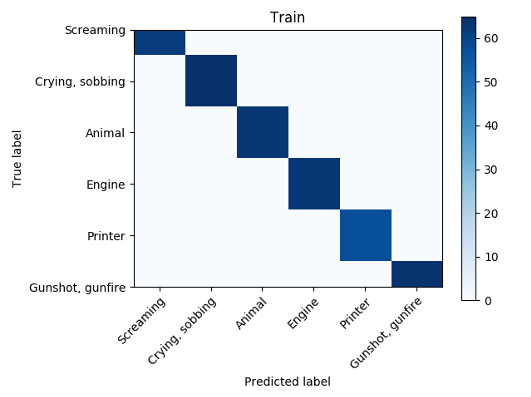
\includegraphics[width=0.5\linewidth]{wav_train}%
			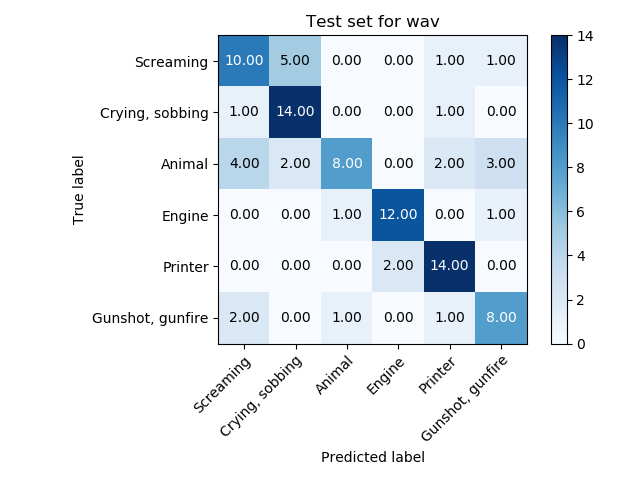
\includegraphics[width=0.5\linewidth]{wav_test}
			\subcaption{Confusion matrices when embeddings are extracted from audio files}
		\end{subfigure}
		\vskip\baselineskip
		% Start with figure tfrecord
		\begin{subfigure}[b]{\textwidth}
			\centering
			\captionsetup{justification=centering}
			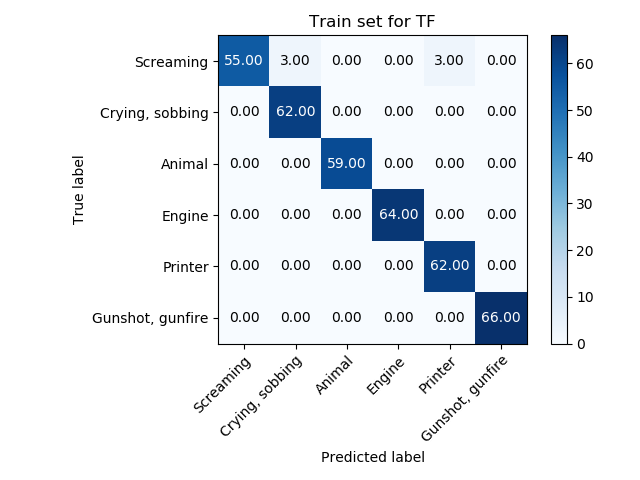
\includegraphics[width=0.5\linewidth]{tfrecord_train}%
			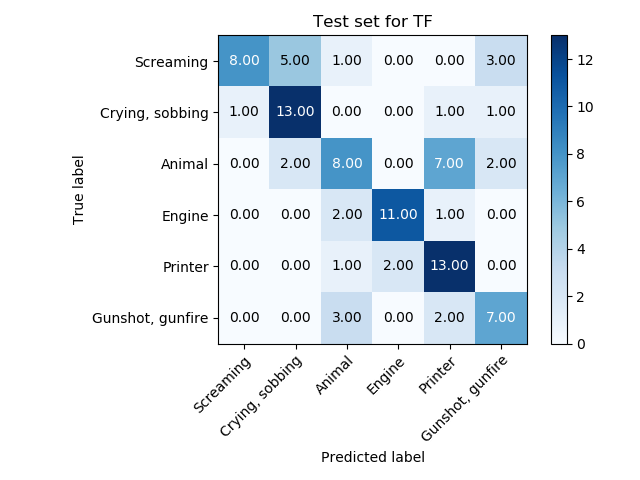
\includegraphics[width=0.5\linewidth]{tfrecord_test}
			\subcaption{Confusion matrices when embeddings are taken from .\textit{tfrecord} files}
		\end{subfigure}
		\caption{Confusion matrices}
		\label{fig:mesh7}
	\end{figure}

	% Accuracy values train and test
	\begin{table}[h]
	\begin{center}
		\centering
		\begin{tabular}{|| m{7em} | m{7em} | m{7em} ||}
			\hline
			format / subset & \textbf{Train} & \textbf{Test} \\
			\hline\hline
			\textbf{Audio file} & 1.0 & 0.79 \\
			\hline
			\textbf{.\textit{tfrecord}} & 1.0 & 0.72 \\
			\hline
		\end{tabular}
	\end{center}
	\caption{Accuracy values for audio and .\textit{tfrecord} files}
	\label{table:5}
	\end{table}

	\doubt{For the training phases, it can be appreciated that there is clearly an overfitting since the accuracy is perfect. This means that the \acrshort{nn} stop improving its capacity of learning how to solve the problem in a certain moment of the training task. Instead, it does learn some behaviour pattern that the training data follows. This impacts negatively in the model since the new data that the system will have to learn from will look different and will not follow these same rules \cite{Jabbar2015}}. In spite of this result, we did not give it so much importance since we just wanted to prove with this experiment the likeness between the two types of data which can be appreciated due to the similarity of both metrics results.
	
\subsubsection{\acrlong{tsne}}
	
	Apart from the classification exercise, we wanted to see if by plotting the data samples we were really able to identify or appreciate some common patterns. In our problem, each of our samples is characterized by a matrix of features with 128 columns, which means that were are working with data belonging to high-dimensional space. Visualizing this type of data has always been a case of study for many different fields. Plenty methods have been published so as to find a solution for this task. Some of the most accepted methods consists on reducing the dimensionality of the data so this can be transformed from the high-dimensional space to a lower one and can be visualize in a common scatter plot of 2D or 3D. In particular, these techniques rely on the idea that a multivariate sample denoted as $x_i = [x_{i1},..., x_{in}]^T$ and considered to be a point that corresponds to a $n-dimensionality$ space, a $d-dimensionality$ space can be found, so that $d < n$, in which the data \doubt{is included}. If this is possible, then the observations can be transformed to this lower dimensional space $d$ without any loses \cite{Kaski2011}. 
	
		% Architecture of model of user interact system
	\begin{wrapfigure}{R}{0.4\textwidth}
		\centering
		\captionsetup{justification=centering}
		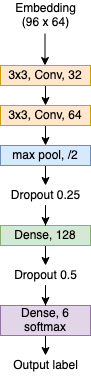
\includegraphics[scale=0.6]{try-wav-tf}
		\caption{Architecture to see how the different embeddings work}
		\label{fig:mesh5}
	\end{wrapfigure}
	
	One of the most common and antique reduction methods is the one known as \acrfull{pca}. This follows the idea previously explained. It specifically wants to extract the \textit{important} information of the original data by and transform them in a set formed by orthogonal variables which are actually known as principal components. This is done by multiplying the matrix data $X$ by a projection matrix $Q$ that contains the coefficients of the linear combinations that let perform the conversion. The projections must be orthogonal from each other and they represent the data maximum variance in descending order, being the first component the one with largest variance \cite{Abdi2010}. In fact, each of the projections correspond to an eigenvector in descending order following the value of the eigenvalue. So, the first component will be the eigenvector with the highest eigenvalue. It has been proved to be one of the most reduction dimensionality techniques nowadays. Its use is completely accepted and it is implemented in many famous software libraries. However, it presents some limitations. One of them consists on just considering linear combinations of the original data. When the relation is non-linear, a dimensionality reduction with this technique may result in a loss of information \cite{AmatRodrigo2017}. 
	
	When the relation between the different subspaces cannot defined as linear, there have been developed other methods with such as \acrfull{tsne}. This algorithm appears as an extension of the previously developed \acrfull{sne} \cite{Hinton2003}. Both are based on the same idea of a new way of measuring the similarity between samples. Instead of comparing two observations, let's call them $x_i$ and $y_j$, by computing the euclidean between them, this is done by calculating the conditional probability $p_{j|i}$ of $x_j$ being picked as a neighbour of $x_i$ considering that the samples belong to a Gaussian distribution centered at $x_i$.Its depends on how far the samples are from each other, i.e., it is high when they are close and minimum when there are totally separated \cite{VanDerMaaten2008}. Apart from this, two analogous observations are created in the subspace of lower-dimensionality, $y_i$ and $y_j$, and conditional probability $q_{j|i}$ is computed in this situation. It is important that, for $y_i$ and $y_j$ to be faithful representations of $x_i$ and $x_j$, both conditional probabilities must be equal.
	
	In order to calculate the probabilities, an crucial factor is the variance of the Gaussian distribution. There is no one unique value for this parameter, so \acrshort{tsne} performs a binary search so as to find the optimal one \cite{AmatRodrigo2017}. This is also influenced by what is called the perplexity. This can be defined as an assumption of the number of adjacent neighbours for each point. It is a value that is fixed by the user, but it usually is comprehend in a range from 5 to 50 \cite{VanDerMaaten2008}. 
	
	There are several considerations that should be known before looking at a representation of data from this algorithm \cite{Wattenberg2016}. Actually, it is not an easy task to understand this kind of plots, since the distance between points in the new subspace are not related to the real euclidean distance, which has been denoted as "The Crowding Problem" \cite{VanDerMaaten2008}. This means that the groups cannot be interpreted as real collections of data in the the original dimension. However, in order not to misunderstand the data distribution, a couple of visualizations varying the parameters usually tend to be done so the conclusions can be based on more than one result. In figure \ref{fig:mesh8} is shown ten \acrshort{tsne} outputs, five for each type of data for diverse values of perplexity from 2 to 50.
	
	% Four confussion matrices
	\begin{figure}[ht]
		% Whole figure
		\captionsetup{justification=centering}
		\begin{subfigure}[b]{\textwidth}
			% Start with figure wav
			\centering
			\captionsetup{justification=centering}
			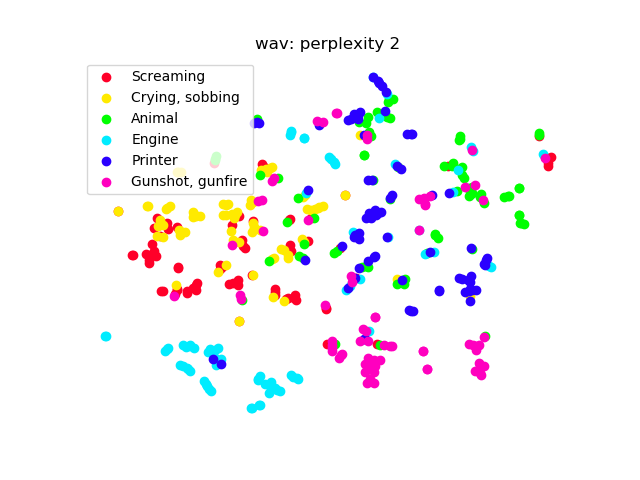
\includegraphics[width=0.2\linewidth]{wav-perp-2}%
			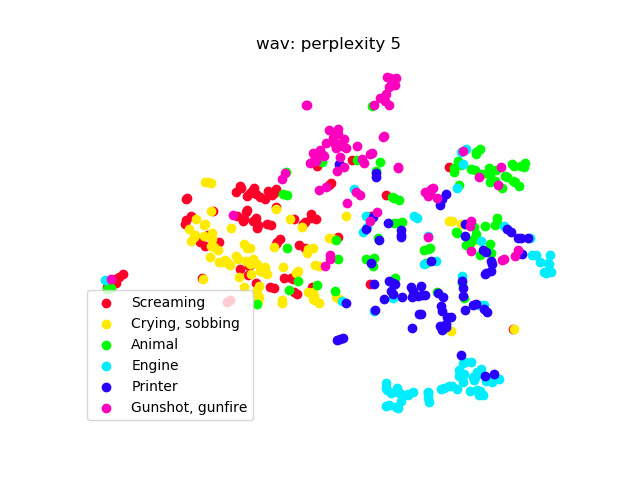
\includegraphics[width=0.2\linewidth]{wav-perp-5}%
			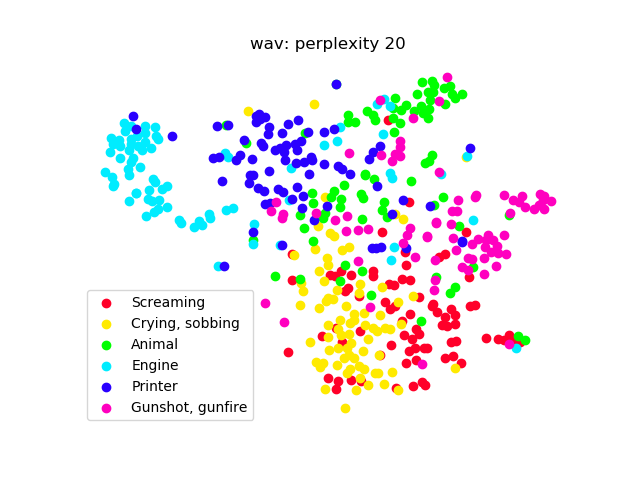
\includegraphics[width=0.2\linewidth]{wav-perp-20}%
			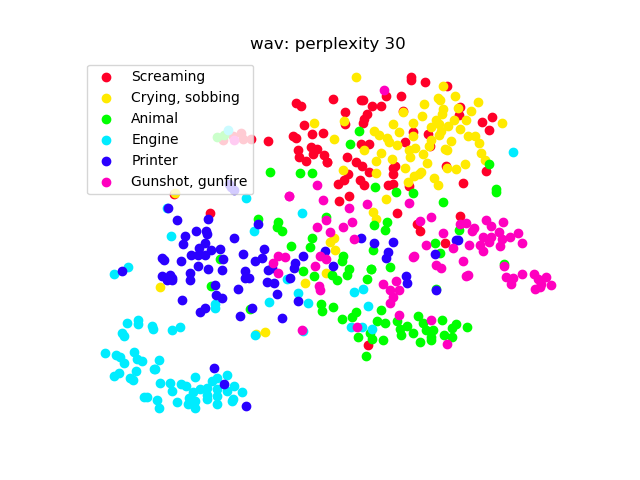
\includegraphics[width=0.2\linewidth]{wav-perp-30}%
			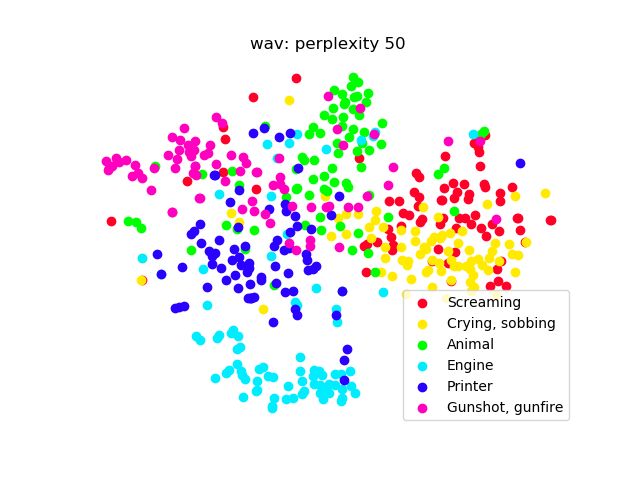
\includegraphics[width=0.2\linewidth]{wav-perp-50}
			\subcaption{From audio files}
		\end{subfigure}
		\vskip\baselineskip
		% Start with figure tfrecord
		\begin{subfigure}[b]{\textwidth}
			\centering
			\captionsetup{justification=centering}
			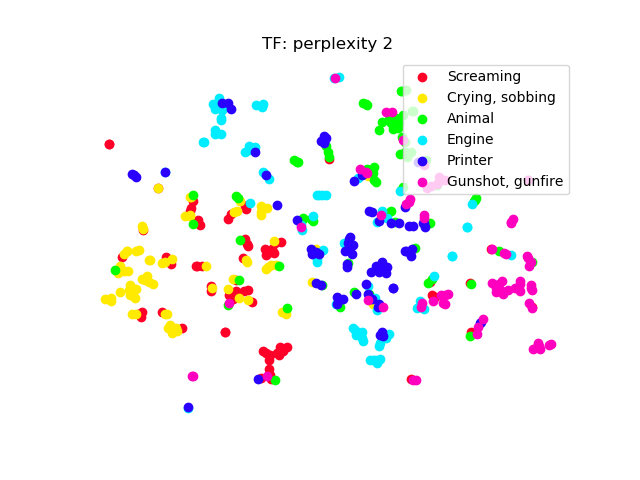
\includegraphics[width=0.2\linewidth]{TF-perp-2}%
			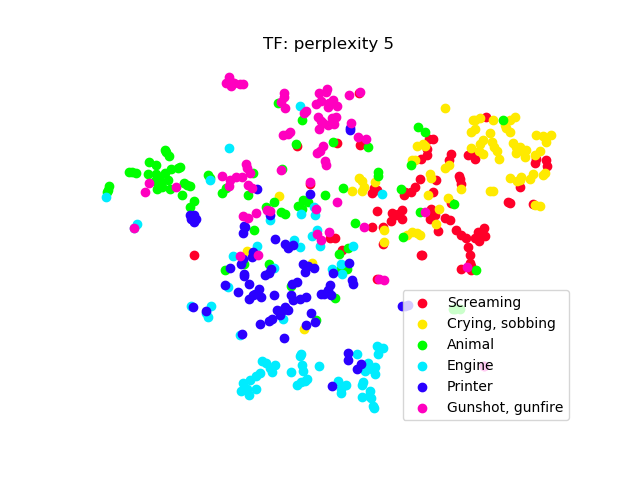
\includegraphics[width=0.2\linewidth]{TF-perp-5}%
			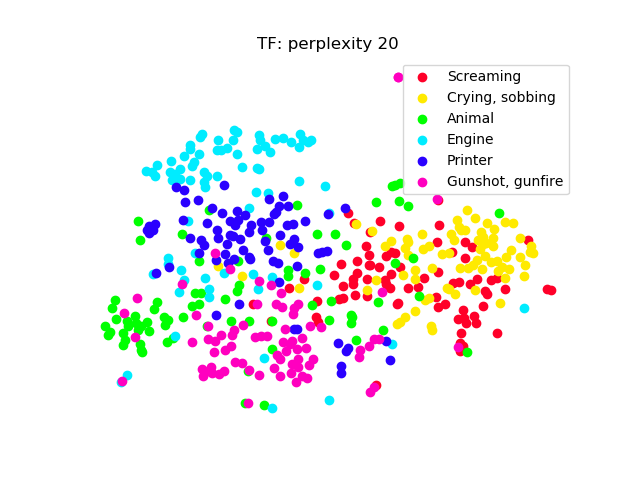
\includegraphics[width=0.2\linewidth]{TF-perp-20}%
			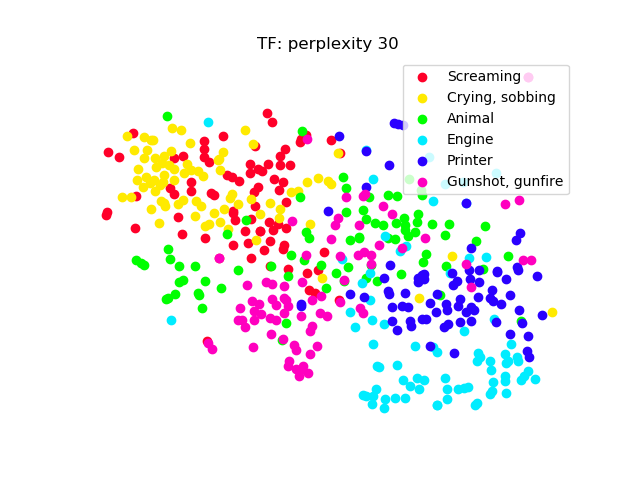
\includegraphics[width=0.2\linewidth]{TF-perp-30}%
			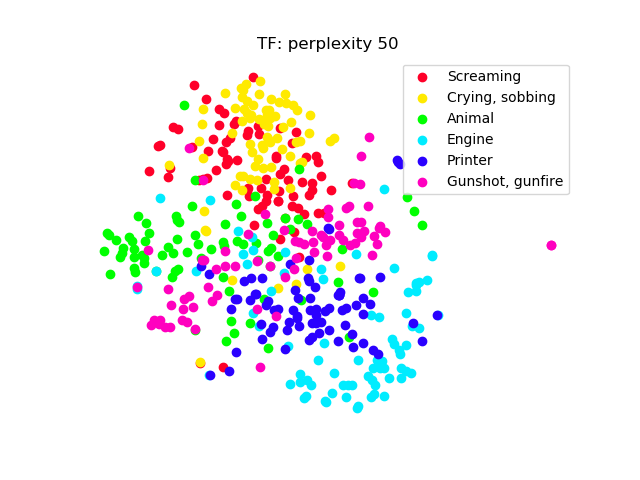
\includegraphics[width=0.2\linewidth]{TF-perp-50}
			\subcaption{From .\textit{tfrecord} files}
		\end{subfigure}
		
		\caption{t-SNE results from both formats with a legend that shows the labels of the data in the original 128D space}
		\label{fig:mesh8}
	\end{figure}
	
	The selection of the perplexity value depends on the number of observations per class \cite{Wattenberg2016}. Since our subset has 80 samples for each category, we can consider that a proper value is 20 or 30. As we can see, a frontier cannot be extracted among the different labels, but we can see some grouping patterns in the data that correspond to the original labelling and helps us to confirm the similarity for the two different given types. It is true that this method should never use as an algorithm of clustering itself, but it is a good resource as a backing strategy to other results, as in this case. 
	
	


	
	
	
	
	

	
	
	

	
	
	
	
	
	
	
	
	